\subsection{Etude du lien entre âge et habitudes alimentaires}

\subsubsection{Préparation des données}

Nous avons ensuite voulu etudier le lien entre l'âge et les habitudes alimentaires.
Cepandant, la valeur du champ âge est directement l'âge, ce qui représente trop de catégories (une vingtaine) par rapport au nombre d'individus présent dans le jeu de données ($500$).
Nous avons donc décidé de répartir les individus en tranches d'âges: les $18-22$, $22-26$, $26-30$ et $30+$.
Nous pouvons maintenant voir dans le tableau de contingence en figure \ref{tab:contTableAgeDietary} que le nombre d'individu est suffisament élevé dans chaque catégorie pour pouvoir faire une AFC ayant du sens.

\begin{figure}[!h]
\begin{center}
  \begin{tabular}{|c|c|c|c|}
    \hline 
    & \multicolumn{3}{|c|}{Dietary Habits}\\ 
    \hline
    Age & Healthy & Moderate & Unhealthy \\ 
    \hline 
    18-22 & 35 & 39 & 42 \\ 
    \hline 
    22-26 & 36 & 34 & 43 \\ 
    \hline 
    26-30 & 41 & 34 & 48 \\ 
    \hline 
    30+ & 49 & 65 & 36 \\ 
    \hline
  \end{tabular}
\end{center}
\caption{Table de contingence entre les habitudes alimentaires et les tranches d'âges}
\label{tab:contTableAgeDietary}
\end{figure}

\subsubsection{Test Chi-deux}

Après exécution du test Chi-deux, la p-valeur obtenue est de $\approx6\%$ ce qui et au dessus de la p-valeur usuellement utilisée pour ce test, mais n'est pas non plus très éloigné.
Ainsi, nous avons quand même décidé de poursuivre l'analyse car cette p-valeur semble tout de même indiquer au moins une faible corrélation entre les deux variables.

\subsubsection{Valeurs propres et cercle des corrélations}

Après exécution de l'AFC, les deux composantes principales obtenues expliquent $100\%$ de la variance, avec la première en expliquant $\approx 97\%$.
Ainsi, la quasi totalité des corrélations seront montrées par la première composante, soit l'axe des abscisses du cercle des corrélations donné en figure \ref{fig:corrAgeDietary}.

\begin{figure}[!h]
  \begin{center}
    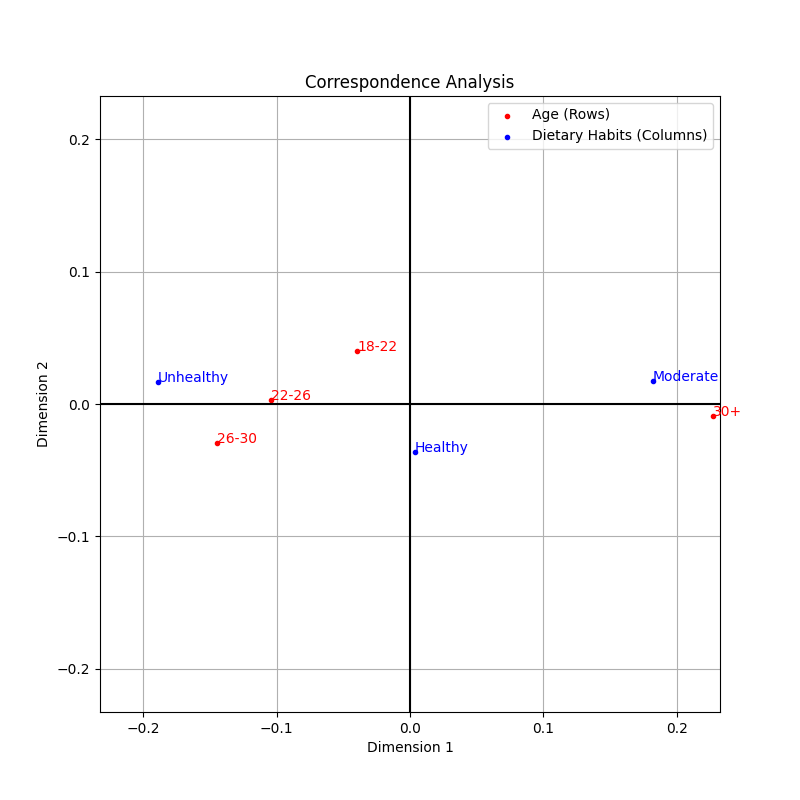
\includegraphics[width=0.55\textwidth]{Images/Age_Dietary_all/Corr_circle.png}
  \end{center}
  \caption{Cercle des corrélations de l'AFC sur les tranches d'âges et les habitudes alimentaires}
  \label{fig:corrAgeDietary}
\end{figure}

Sur la figure \ref{fig:corrAgeDietary}, on peut constater 2 légères tendances\footnote{Nous insistons vraiment sur le fait que ces corrélations sont faibles et ne représentent qu'au plus des légères tendances}:
\begin{itemize}
  \item Les plus de 30 ans ont tendance à avoir une alimentation modérée 
  \item Les 26-30 ans et 22-26 ans tendent quand à eux vers une alimentation plutôt mauvaise pour la santé
\end{itemize}

Cette tendance se confirme en regardant la contribution de chaque catégorie sur les composantes principales.
En effet, comme on peut le voir sur la figure \ref{fig:contribAgeDietary}, la première composante dépend des catégories Moderate et Unhealthy de manière approximativement égale, et la figure \ref{fig:corrAgeDietary} montre en complément que Moderate y contribue positivement et Unhealthy y contribue négativement. 
Ainsi, l'analyse de correspondance a classé les tranches d'ages selon le nombre d'individus ayant un régime modéré moins le nombre d'individus ayant un régime mauvais pour la santé. 

\begin{figure}[!h]
  \begin{center}
    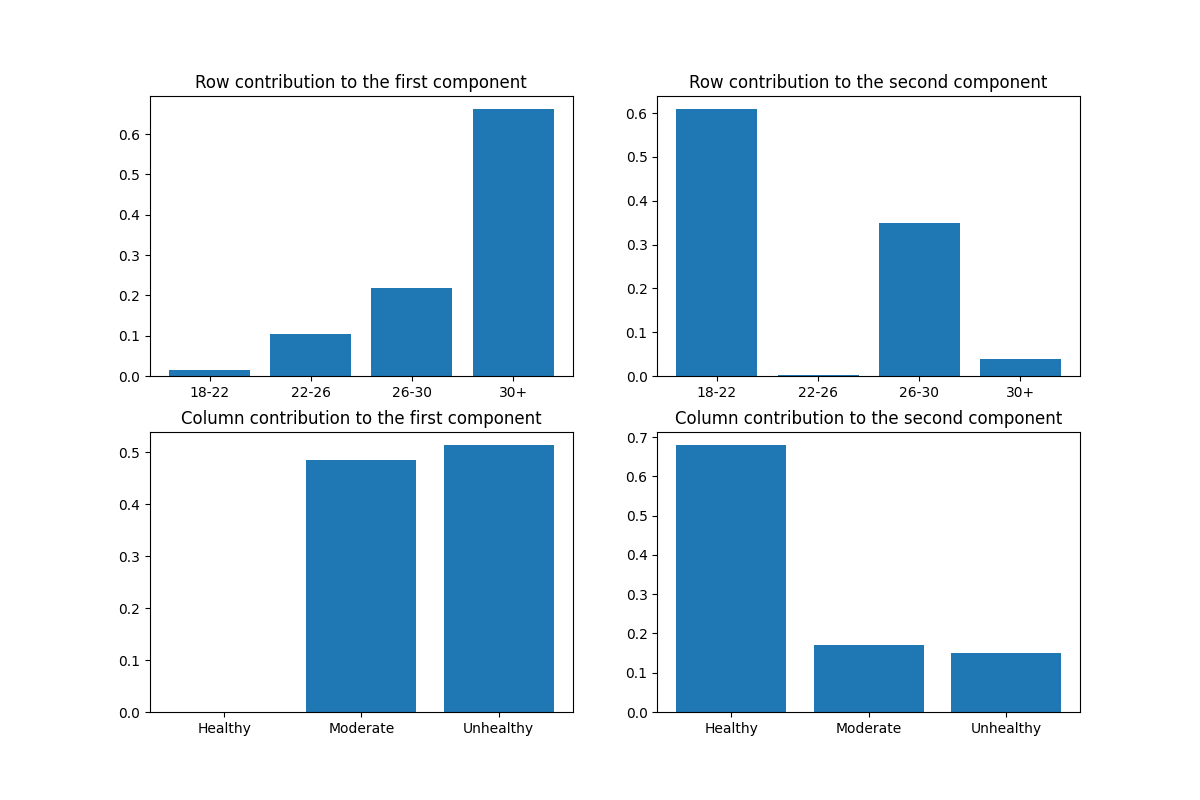
\includegraphics[width=0.95\textwidth]{Images/Age_Dietary_all/RowColumnsContributions.png}
  \end{center}
  \caption{Contribution des catégories dans les composantes principales}
  \label{fig:contribAgeDietary}
\end{figure}

